Struktureller Aufbau des Projektes.

\tikzstyle{myNode20} = [draw=black, fill=black!20,
    rectangle, inner sep=5pt, inner ysep=5pt]
\tikzstyle{myNode15} = [draw=black, fill=black!15,
    rectangle, inner sep=5pt, inner ysep=5pt]
\tikzstyle{myNode10} = [draw=black, fill=black!10,
    rectangle, inner sep=5pt, inner ysep=5pt, text width=5cm]
\tikzstyle{myNode5} = [draw=black, fill=black!5,
    rectangle, inner sep=5pt, inner ysep=5pt, text width=3cm]

\tikzstyle{folderline} = [very thick, dashed]

\usetikzlibrary{fit,positioning}
\pgfdeclarelayer{l1}
\pgfdeclarelayer{l2}
\pgfdeclarelayer{l3}
\pgfsetlayers{l1,l2,l3,main}

\definecolor{col}{HTML}{CBF7FF}
\colorlet{col1}{col}
\colorlet{col2}{col!70}
\colorlet{col3}{col!30}
\colorlet{col4}{col!10}


\tikzstyle{tt} = [font=\ttfamily, left, inner sep=5pt]
\tikzstyle{sub} = [below right=5pt and 50pt of #1.south west, 
                   anchor=north west]
\tikzstyle{des} = [below=2pt of #1.south west, anchor=north west]

\tikzstyle{l4} = [fill=col4, draw=col4!50!black, inner sep=5pt]
\tikzstyle{l3} = [fill=col3, draw=col3!50!black, inner sep=5pt]
\tikzstyle{l2} = [fill=col2, draw=col2!30!black, inner sep=5pt]
\tikzstyle{l1} = [fill=col1, draw=col1!30!black, inner sep=5pt]

\newcommand{\surround}[3]{
  \begin{pgfonlayer}{l#1}
  \node[l#1,fit=(#2) #3, xshift=5pt, yshift=-5pt] (f#2) {};
  \draw[l#1] (#2.south-|f#2.west) -- (#2.south-|f#2.east);
  \end{pgfonlayer}
}

\begin{center}
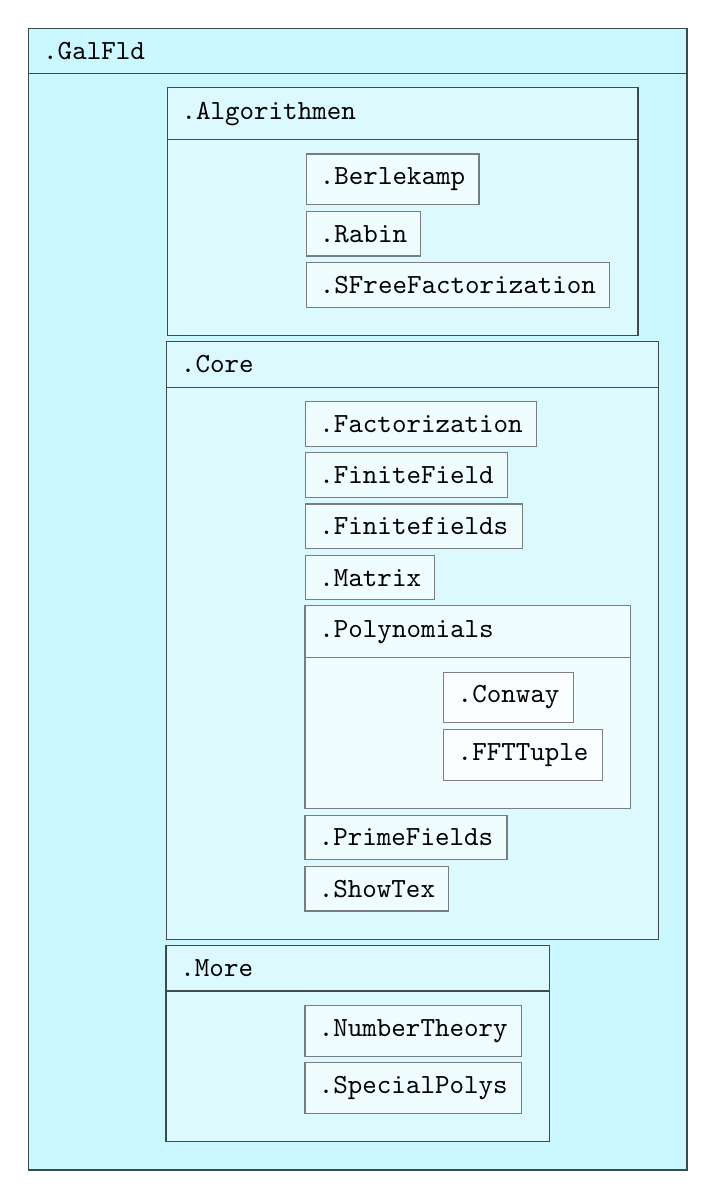
\begin{tikzpicture}

\iffalse

\draw[myNode20] (-2.4,1.4) rectangle (8.4,-11.5);
\draw[myNode15] (-2,0.4) rectangle (8,-8.4);
\draw[myNode15] (-2,-8.6) rectangle (8,-11.4);
\draw[myNode15] (-2,-11.6) rectangle (8,-13.4);
\draw[myNode10] (2.5,-0.5) rectangle (13,-3.5);

\node[text width=3cm] (GalFld) at (0,1) [] {\texttt{GalFld.hs}};
\node[text width=3cm] (Core) at (0,0) [] {\texttt{Core.hs}};
  \node[myNode10] (ShowTex) at (5,0) [] {\texttt{ShowTex.hs}};
  \node (Polynomials) at (5,-1) [] {\texttt{Polynomials.hs}};
    \node[myNode5,dotted,very thick] (FFT) at (11,-1) [] {\texttt{FFT.hs}};
    \node[myNode5,dotted,very thick] (FFTTuple) at (11,-2) {\texttt{FFTTuple.hs}};
    \node[myNode5,dotted,very thick] (Conway) at (11,-3) {\texttt{Conway.hs}};
  \node[myNode10] (FiniteField) at (5,-4) [] {\texttt{FiniteField.hs}};
  \node[myNode10] (PrimeFields) at (5,-5) [] {\texttt{PrimeFields.hs}};
  \node[myNode10] (FiniteFields) at (5,-6) [] {\texttt{FiniteFields.hs}};
  \node[myNode10] (Matrix) at (5,-7) [] {\texttt{Matrix.hs}};
  \node[myNode10] (Factorization) at (5,-8) [] {\texttt{Factorization.hs}};
\node[text width=3cm] (Algorithmen) at (0,-9) [] {\texttt{Algorithmen.hs}};
  \node[myNode10] (SFreeFactorization) at (5,-9) []
    {\texttt{SFreeFactorization.hs}};
  \node[myNode10] (Berlekamp) at (5,-10) [] {\texttt{Berlekamp.hs}};
  \node[myNode10] (Rabin) at (5,-11) [] {\texttt{Rabin.hs}};
\node[text width=3cm] (More) at (0,-12) [] {\texttt{More.hs}};
  \node[myNode10] (NumberTheory) at (5,-12) [] {\texttt{NumberTheory.hs}};
  \node[myNode10] (SpecialPolys) at (5,-13) [] {\texttt{SpecialPolys.hs}};

\fi


\node[tt] (1) {.GalFld};
\node[tt, sub=1] (1-1) {.Algorithmen};
\node[l3,tt, sub=1-1] (1-1-1) {.Berlekamp};
\node[l3,tt, des=1-1-1] (1-1-2) {.Rabin};
\node[l3,tt, des=1-1-2] (1-1-3) {.SFreeFactorization};
\surround{2}{1-1}{(1-1-1) (1-1-2) (1-1-3)}

\node[tt, des=f1-1] (1-2) {.Core};
\node[l3,tt, sub=1-2] (1-2-1) {.Factorization};
\node[l3,tt, des=1-2-1] (1-2-2) {.FiniteField};
\node[l3,tt, des=1-2-2] (1-2-3) {.Finitefields};
\node[l3,tt, des=1-2-3] (1-2-4) {.Matrix};
\node[tt, des=1-2-4] (1-2-5) {.Polynomials};

\node[l4,tt, sub=1-2-5] (1-2-5-1) {.Conway};
\node[l4,tt, des=1-2-5-1] (1-2-5-2) {.FFTTuple};
\surround{3}{1-2-5}{(1-2-5-1) (1-2-5-2)}

\node[l3,tt, des=f1-2-5] (1-2-6) {.PrimeFields};
\node[l3,tt, des=1-2-6] (1-2-7) {.ShowTex};

\surround{2}{1-2}{(1-2-1) (f1-2-5) (1-2-7)}

\node[tt, des=f1-2] (1-3) {.More};
\node[l3,tt, sub=1-3] (1-3-1) {.NumberTheory};
\node[l3,tt, des=1-3-1] (1-3-2) {.SpecialPolys};

\surround{2}{1-3}{(1-3-1) (1-3-2)}

\surround{1}{1}{(f1-1) (f1-2) (f1-3)}

\end{tikzpicture}
\end{center}
